% EAMAN: The y range of these two figures should be the same. The text on axis should be larger. Preferably, box the plots too.
%EAMAN: these plots add little information and are obsolete now as the trivialness is missing for a large portion of coins, and shows no significance for the coins that have that data. 

Speculative bubbles are perceived to periodically take over markets \cite{garber2001famous}.
Going back at least to the \emph{South Sea} bubble in the early 18\textsuperscript{th} century, well-informed parties  have invested knowingly in bubbles, and found it profitable \cite{temin2004riding}.
Today, the public notoriety of Bitcoin, together with its massive price increases and their associated publicity lead to an explosion of attempts to create ``the next Bitcoin''.
Collectively, these currencies are often referred to as ``cryptocurrencies'' or ``cryptocoins'' or simply ``coins'', and a vibrant set of exchanges have emerged where these are traded, either for each other or money.
The majority of these coins have no possible future value in the long term, and their markets would appear to be driven largely by speculation.
Many of them appear to be nothing but attempts at turning a quick profit from inflating the implied valuation of a coin shortly after creating it.
This is driven by the extremely low cost and effort required to create a new coin, with most being minimal changes to parameters and branding of a pre-existing codebase.

Those who make and trade these coins communicate largely online, and much of their activity is concentrated on public forums. 
Moreover, price and volume data from the exchanges is freely available and widely aggregated\footnote{Exchanges are however largely unregulated, often anonymous, and there is no way to account how much of reported volumes are manipulation attempts. The existence of attempts at arbitrage between them places some bounds on how blatantly the data can be manipulated for prices, but volumes are impossible to assess. },
%JULIAN: Whole footnote is one extra-long sentence!
and public source code to all cryptocoins is the community norm. This makes cryptocoins
an ideal lens through which to study the social life of a ``market mania'' \cite{cosma2008}.
Such a study is valuable both as a means of understanding the dynamics of bubbles themselves, but also from a computational social science perspective, to understand the ecosystem and lifecycles of these online communities.
%Such a study can serve in the computational social sciences a role analogous to that of lesion studies do in neuropsychology.
%JULIAN: Not obvious to me what the above analogy is without further explanation.
%EAMAN: commented out.

We present a study of a large number of cryptocurrency ecosystems, 
using a novel dataset that combines measures derived from social networks of users interacting in online cryptocurrency forums and market data aggregated over dozens of exchanges.
From forums, we identify the users who introduce each coin to the community and build measures of their structural position in the network based on
their engagement patterns in forum threads \emph{before} the coin is ever traded (usually within a few days after their announcement on the forum).
In this way, we identify 626 coins that are announced by users of the forum and can be mapped to price and volume data from the exchanges.
Next, from price and transaction volume data, we build measures of speculation that quantify the size of the bubble resulting from trading activity on each coin. 
Many of the new coins announced on the forums experience a frenzied period of rising prices as users are looking for the next Bitcoin. However in many of these cases, prices sharply fall as soon as the users discover the shortcomings in the design, learn about the lack of real innovation or simply because first adapters observe about a weak community response to the new coin. For this reason, the cryptocurrency ecosystem presents a great opportunity for studying the mechanisms behind formation of bubbles, due to the abundance of such cases.


%\begin{figure}
%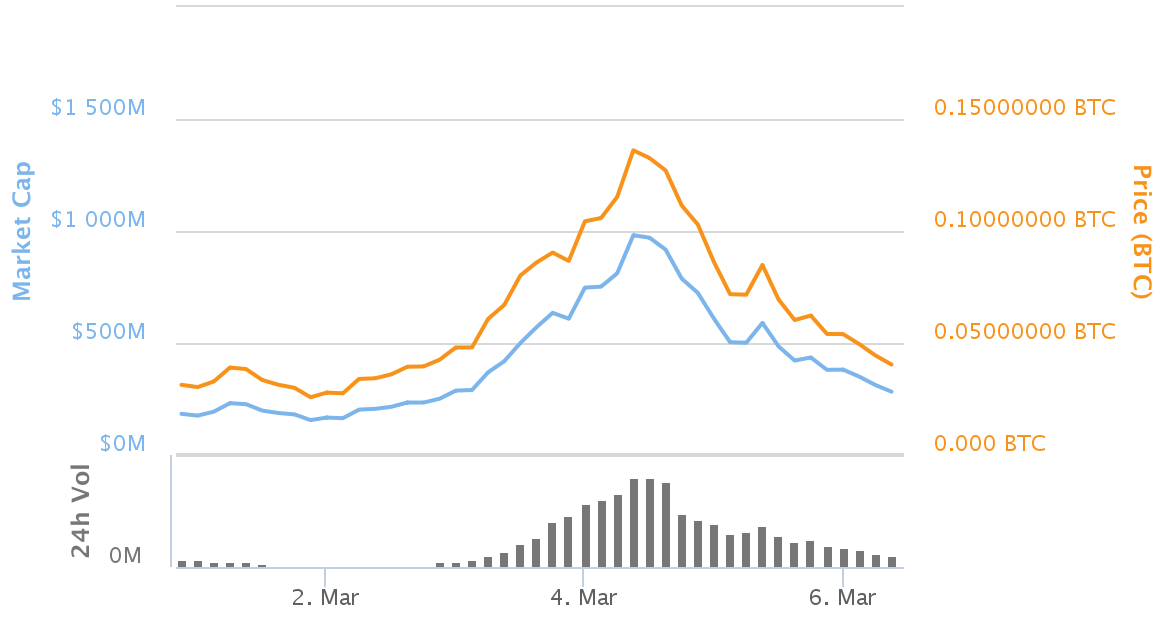
\includegraphics[width=\columnwidth]{AuroraCoin}
%\end{figure}

\begin{figure}
\centering
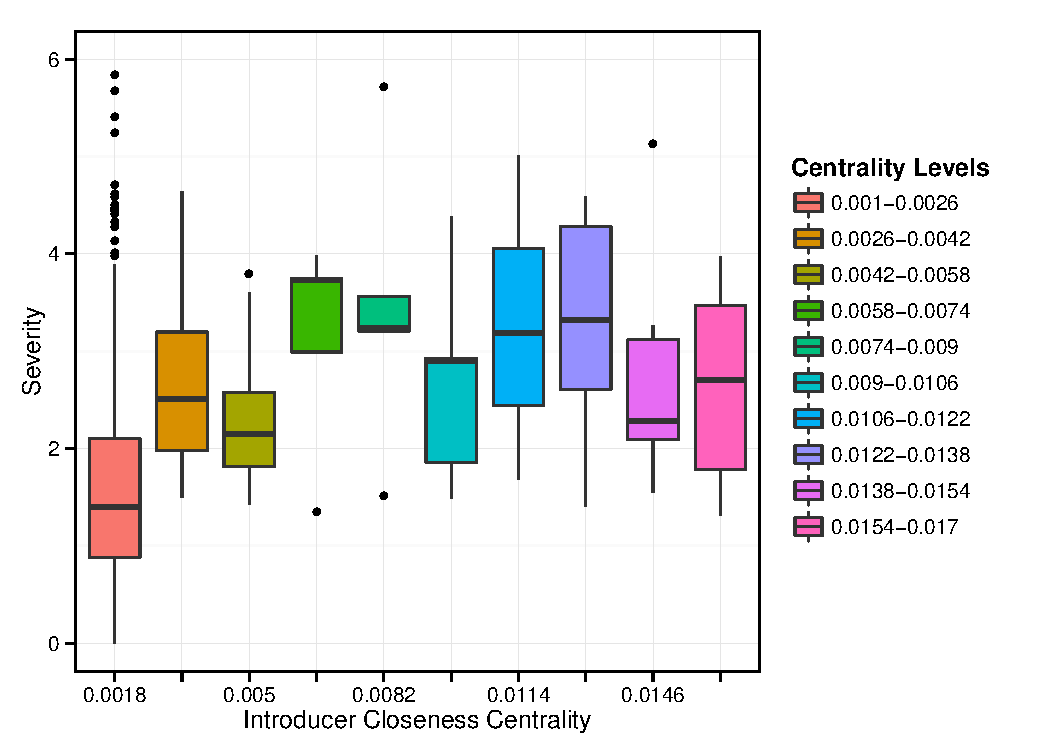
\includegraphics[width=1.1\columnwidth]{severity_boxplot.pdf}
\label{severity_boxplot}
\caption{The bubble severity vs. coin introducer closeness centrality in the discussion network. Centrality of asset introducer is the most predictive variable for bubble severity in our final model. It has a stronger relationship with bubble severity than its magnitude.}
\end{figure}

While the mechanisms that drive bubbles have been studied both theoretically 
\cite{abolafia1988enacting,earl2007decision,bakker2010social,harras2011grow}
and experimentally
\cite{moinas2013bubble},
% in the lab, 
studying the social networks of those promoting the asset has not been previously possible due to the lack of an exhaustive dataset. To the best of our knowledge, our work is the first to analyze the role that the global structural features of the communication network, such as the position of certain stakeholders, can play in promoting the asset.
While the magnitude of the assets traded in our study is small relative to most financial and commodity markets, it is nevertheless much larger than
%JULIAN: Found this sentence a bit funny, not that I could improve upon it
%EAMAN: kudos nikete
any plausible experiment in an academic environment.
For example, the largest bubble in our dataset, AuroraCoin, reached a valuation of one billion USD in March 2014,
with reported daily trading volumes of 6.8M USD. It shed 90\% and 99\% of its value in a week and well under a year, respectively.
To provide some context, this is equivalent to one quarter of Iceland's entire foreign exchange reserves in 2014 \footnote{4.1 Billon USD, The World Bank, Global Economic Monitor, accessed October 2015}, the population of which AuroraCoin promoters claimed they would distribute half of the coins to.

Using price and volume data, we construct measures of both the \textbf{magnitude} and the \textbf{severity} of bubbles.
These are defined formally in our variable section %\ref{variables_nikete},
but their intuition is that we say the magnitude of a bubble is large when a high volume of trades measured in dollars happens,
%JULIAN: Does it make a difference what it's measured in?
%EAMAN: yes. a lot
while a coin has a severe bubble if investing a fixed amount leads to losing a large proportion. 
By considering the community structure that exists in the forums before a coin is traded, we are able to predict a substantial fraction of the variation in the severity and a smaller fraction of the magnitude of the resulting bubble.
This is a challenging task as models that rely on either simple activity or network metrics show almost no predictive out-of-sample power, and are unable to explain even 1\% of the variation in either tasks,
while our best model performs an order of magnitude better in both tasks and does not even use the forum activity information after trading on each coin starts. 
%JULIAN: R^2 of 0.1 (if I interpret correctly) doesn't sound impressive until you've argued the fundamental difficulty of the problem, you might wait to mention such numbers.
%JULIAN: Would sound more impressive if you just said "it performs an order of magnitude better"
%EAMAN: sure..
The main driver of our explanatory power is the centrality of users in the directed communication network derived from the forum. As it can be seen in Figure ~\ref{severity_boxplot}, the severity of the bubbles increase with the centrality of the users who introduce new coins to the community. However, both the severity and the magnitude of bubbles decrease with the seniority of such users.
%JULIAN: Above sentence is tough to parse, but kind of an important one.
%EAMAN: tried fixing. how does it sound?

%EAMAN: commented out. repetion of what is said below.
%This effect appears to be mediated by whether a coin involves a nontrivial technological innovation, the direction of the interaction reversing depending on whether it relates to magnitude or severity.

%EAMAN: commented out. trivialness shows no significance. Moreover, in the plots above the betas well overlap when using their se's, so the below statement is possibly wrong.
%Interestingly this effect is concentrated in different ways depending on whether the coin software is more than a trivial modification to existing code base: as shown in Figure \ref{volume_severity_centrality} trivial coins have more severe bubbles the more central their introducers are, while volume is greater the more central the introducer of a nontrivial coin is.

%Methodologically the free parameters in the way we do the weights on the weighted graph  is horrible, a million free parameters get introduced. follow up work for another paper: do some unsupervised feature learning over the dam forums threads to build the network; use some internal validity metric . Find political way of saying this in future work.

